\section{Model Exercise 3-2: Constant normal stiffness (CNS) direct shear test}
\label{sec:mex08}\index{Constant Normal Stiffness (CNS) experiment}
%------------------------------------------------------------------------------
\Authors{Daniel P\"otschke, Thomas Fr\"uhwirt et al.}
%------------------------------------------------------------------------------
\subsection{Experimental set-up}
%------------------------------------------------------------------------------
\begin{figure}[!ht]
\begin{center}
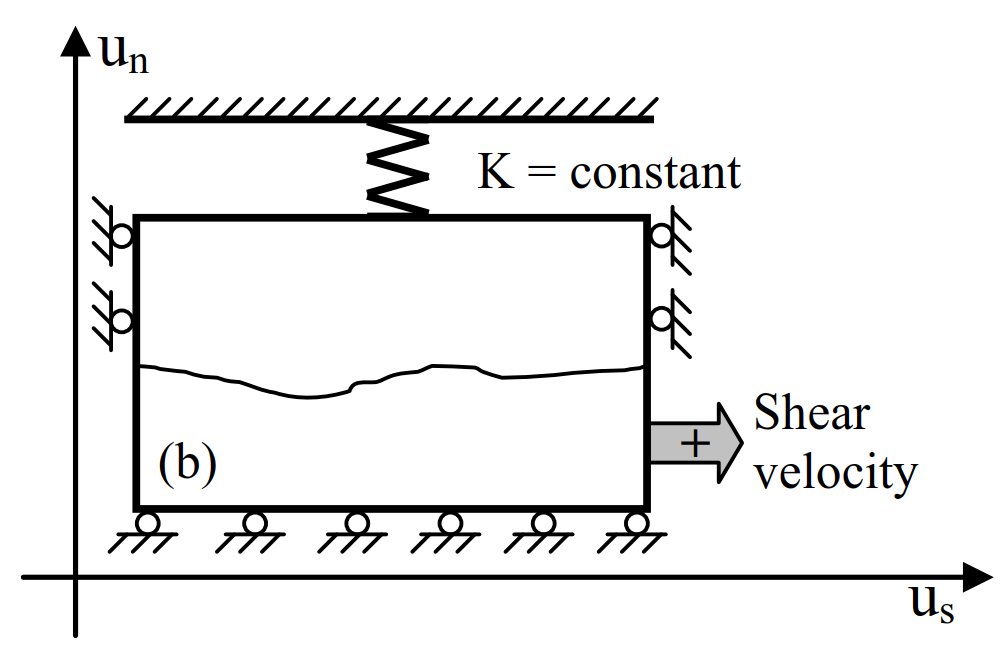
\includegraphics[width=0.5\textwidth]{./figures/MEX8_CNS_Nguyen_Thesis.PNG}
\end{center}
\caption{Constant normal stiffness (CNS) direct shear test. (From: \cite{Nguyen2014})}
\label{fig:MEX8_CNS}
\end{figure}

Constant normal stiffness (CNS) direct shear tests follow the same basic principles like CNL tests (\ref{sec:mex07}). Additionally to the initial normal load an extra load is added when the rock joint opens. This situation is comparable to a rock joint in the underground where surrounding rock masses have to be deformed to open a joint. This deformation causes the extra loads. In Fig. \ref{fig:MEX8_CNS} the stiffness term is represented as a spring with a constant stiffness. The difficulty is to estimate this stiffness. If the joint is surrounded by intact rock material it will be higher than for a jointed, weathered surrounding. A CNL test is a CNS test for which the stiffness is zero. This situation marks the lower boundary of the stiffness and is a valid boundary condition for rock joints close to the surface. The upper boundary of the stiffness is the stiffness of the intact rock. The real situation will be somewhere in between this extreme cases.\\
The expected result is that for higher stiffness values the shear forces increase due to the increasing normal load when the joints starts to open.\\
The input data for this model exercise are explained in \ref{DataManMex3-2CNS}. The aim is to use this input to make good back calculations of the lab data. A good modelling approach for CNS tests can also be used for CNL tests by simply setting the stiffness to zero.


%------------------------------------------------------------------------------
\subsection{Model approach}
%------------------------------------------------------------------------------
The model approach basically follows the approach of the CNL test, see \ref{sec:mex07}.\\
Additionally an estimation of the dilatation is needed. The normal stress has to be updated once the dilatation is known. The dilatation is modeled using a geometric approach where the dip angle of the worn surface is used as inclination angle.

%------------------------------------------------------------------------------
\subsection{Results and discussion}
%------------------------------------------------------------------------------
\todod{[TUBAF] Please complete section}
The results show that in the lab testings an entire edge was destructed, see Fig. \ref{fig:MEX3-2_AbrasionPic}. Thus the simulation was done with 2 different scenarios: One with the original geometry and one with an adapted geometry where this edge was manually removed. The orientation of the edge in the left upper or right bottom corner is a result of different definitions using matrices and the plotting as surface or image.\\
\begin{figure}[!ht]
\begin{center}
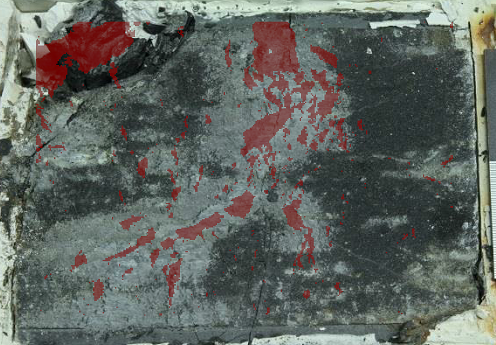
\includegraphics[width=0.5\textwidth]{./figures/MEX3-2_AbrasionPicVsSim.PNG}
\end{center}
\caption{Visual comparison of the destructed areas of the rock joint. Notice the entirely destroyed edge.}
\label{fig:MEX3-2_AbrasionPic}
\end{figure}


Figure \ref{fig:MEX3-2_AbrasionPic} shows a visual comparison between the abrasion visible from the rock surface and the location of damage from the simulation. It can be concluded, that the used FFS approach (\ref{chap:NumPlatf:FFS}) is able to roughly locate the occurrence of abrasion though it is not able to forecast the destruction of a bigger section.\\

\begin{figure}[!ht]
\begin{center}
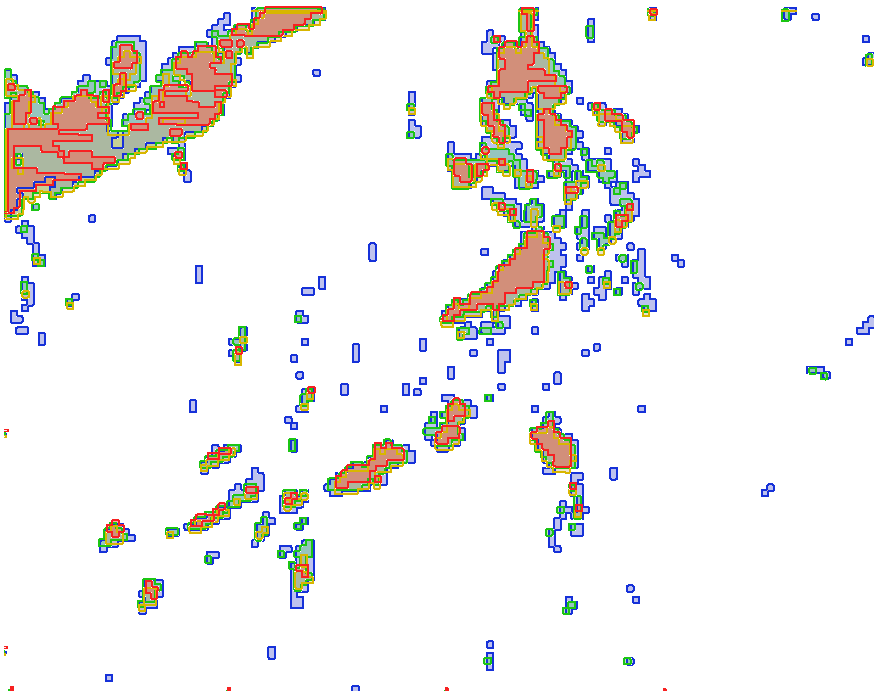
\includegraphics[width=0.5\textwidth]{./figures/MEX3-2_AbrasionDiffStiffness.PNG}
\end{center}
\caption{The destructed area for different stiffness values. The area of destruction increases with the stiffness. \textit{red:} $2\, \unit{MPa}$, \textit{yellow:} $4\, \unit{MPa}$, \textit{green:} $8\, \unit{MPa}$, \textit{blue:} $16\,\unit{MPa}$}
\label{fig:MEX3-2_AbrasionStiffness}
\end{figure}

In Fig. \ref{fig:MEX3-2_AbrasionStiffness} a comparison between the simulated abrasion for different stiffness values during the CNS test series can be seen. As expected the area of damage increases with increasing stiffness. The size of the bigger areas increases and new areas start to develop as well. This result acts as a verification of the code.\\


\begin{figure}
\begin{subfigure}[c]{0.48\textwidth}
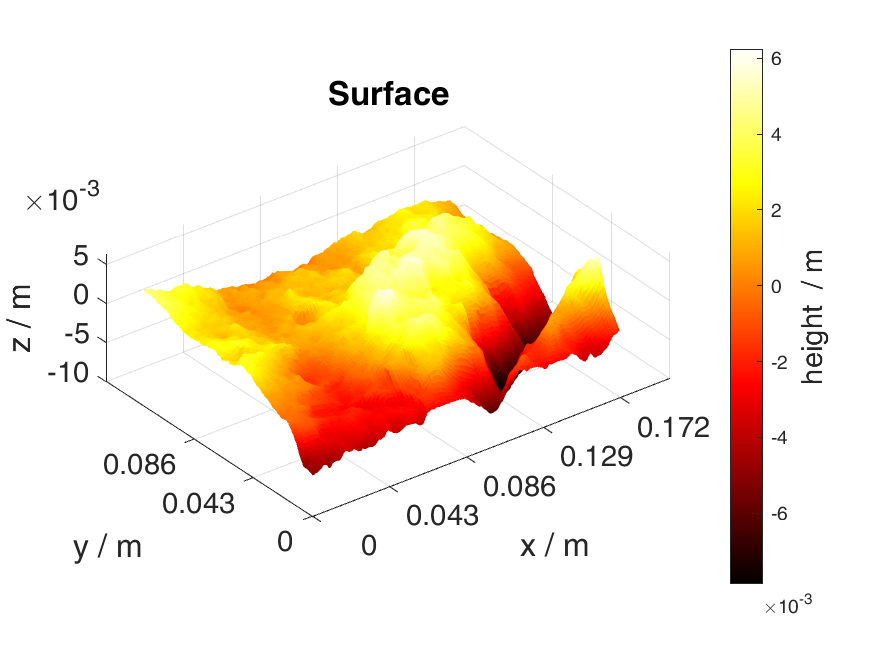
\includegraphics[width=0.99\textwidth]{./figures/MEX3-2_SurfaceOrig.png}
\subcaption{Original geometry}
%\label{fig:}
\end{subfigure}
\begin{subfigure}[c]{0.48\textwidth}
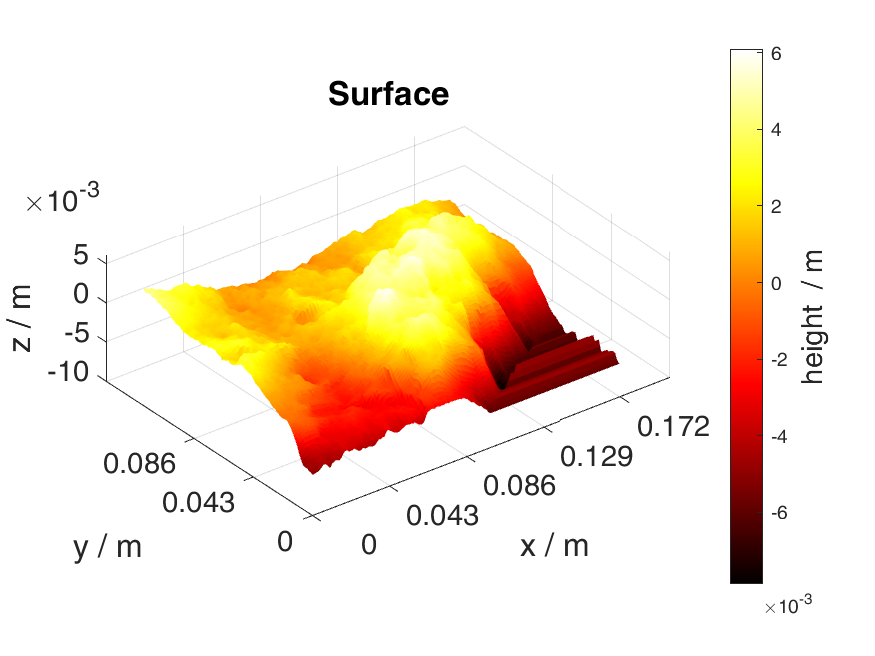
\includegraphics[width=0.99\textwidth]{./figures/MEX3-2_SurfaceWithout.png}
\subcaption{Adapted geometry}
%\label{fig:}
\end{subfigure}
\caption{The used geometries for the CNS test.}
\label{fig:MEX3-2_Surface}
\end{figure}

In Fig. \ref{fig:MEX3-2_Surface} the used geometries for the the original morphology and the adapted one with the destructed edge can be seen. The results are shown for two different stiffness values and for comparison always the result for the original geometry and the adapted geometry are displayed.\\

\begin{figure}
\begin{subfigure}[c]{0.48\textwidth}
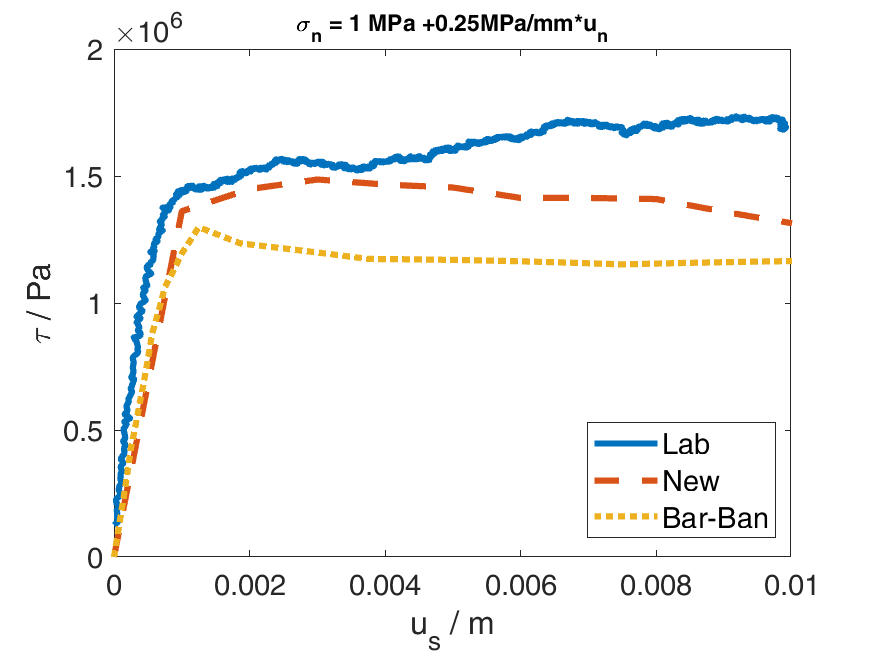
\includegraphics[width=0.99\textwidth]{./figures/MEX3-2_025ShearCurveOrig.png}
\subcaption{Original geometry}
%\label{fig:}
\end{subfigure}
\begin{subfigure}[c]{0.48\textwidth}
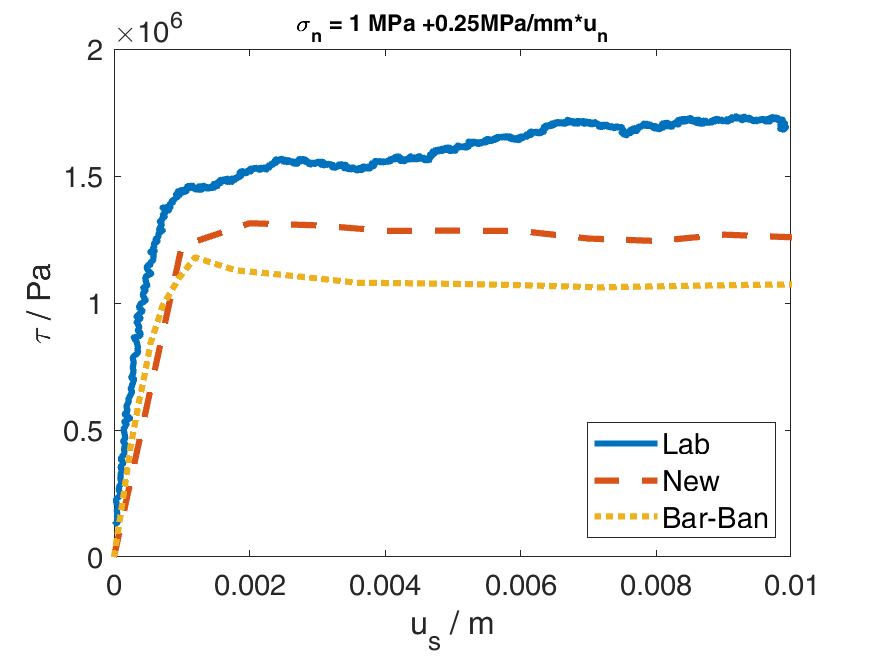
\includegraphics[width=0.99\textwidth]{./figures/MEX3-2_025ShearCurveWithout.png}
\subcaption{Adapted geometry}
%\label{fig:}
\end{subfigure}
\caption{Shear curves for $K_n=0.25\,\unit{MPa}$}
\label{fig:MEX3_2_025ShearCurve}
\end{figure}

\begin{figure}
\begin{subfigure}[c]{0.48\textwidth}
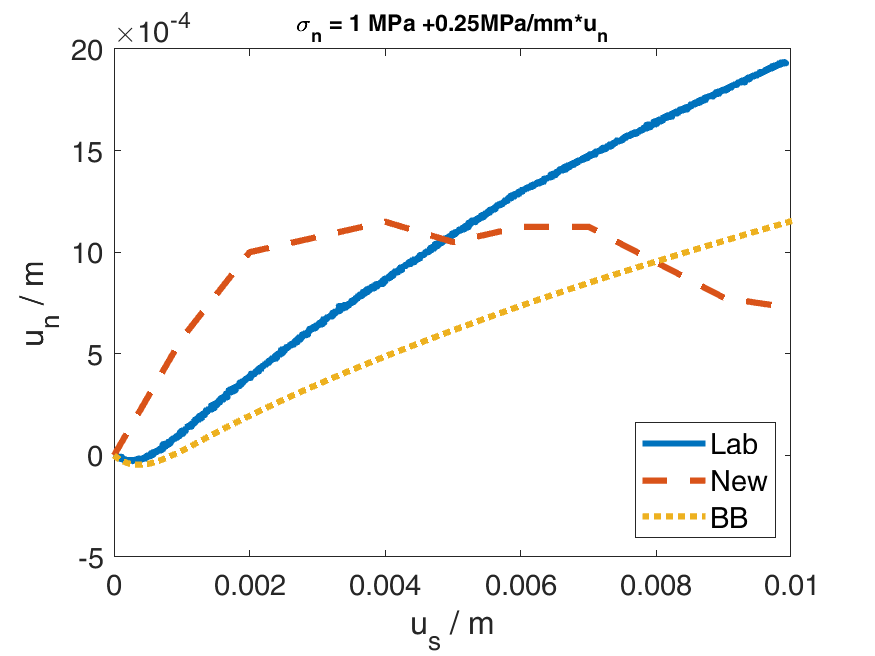
\includegraphics[width=0.99\textwidth]{./figures/MEX3-2_025DilationOrig.png}
\subcaption{Original geometry}
%\label{fig:}
\end{subfigure}
\begin{subfigure}[c]{0.48\textwidth}
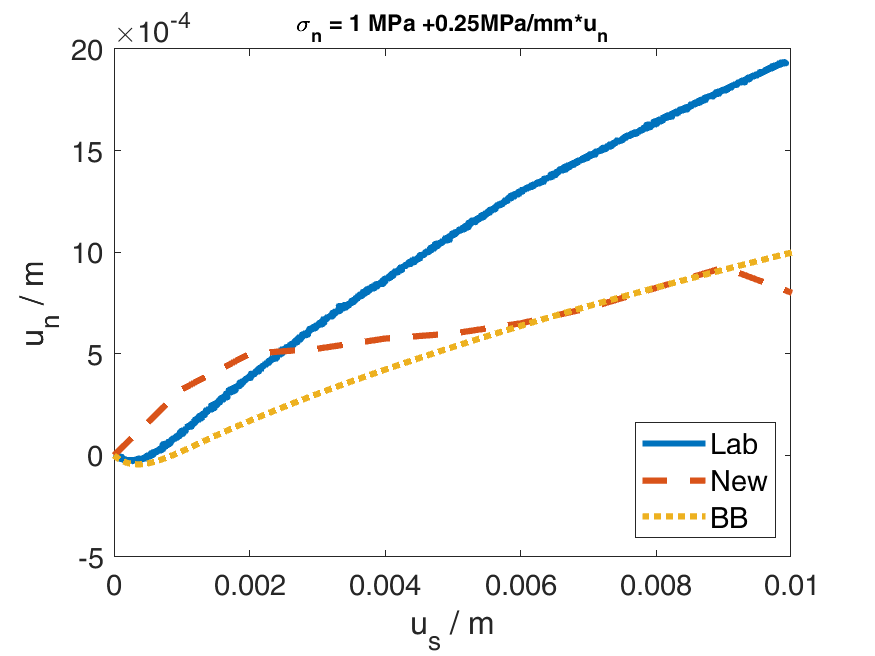
\includegraphics[width=0.99\textwidth]{./figures/MEX3-2_025DilationWithout.png}
\subcaption{Adapted geometry}
%\label{fig:}
\end{subfigure}
\caption{Dilatation curves for $K_n=0.25\,\unit{MPa}$}
\label{fig:MEX3-2_025Dilation}
\end{figure}

In Fig. \ref{fig:MEX3_2_025ShearCurve} and Fig. \ref{fig:MEX3-2_025Dilation} the shear curves and the dilatation curves for a low stiffness value can be seen. The results show that the general trend of the shear curves is similar. On the other hand the dilatation curves are quite poor. Especially the dilatation curves for original and adapted geometry show some differences. In the shear curves this difference is minor because the low stiffness isn't dominating the overall normal stress and as a consequence the shear stress is not too strongly influenced.\\

\begin{figure}
\begin{subfigure}[c]{0.48\textwidth}
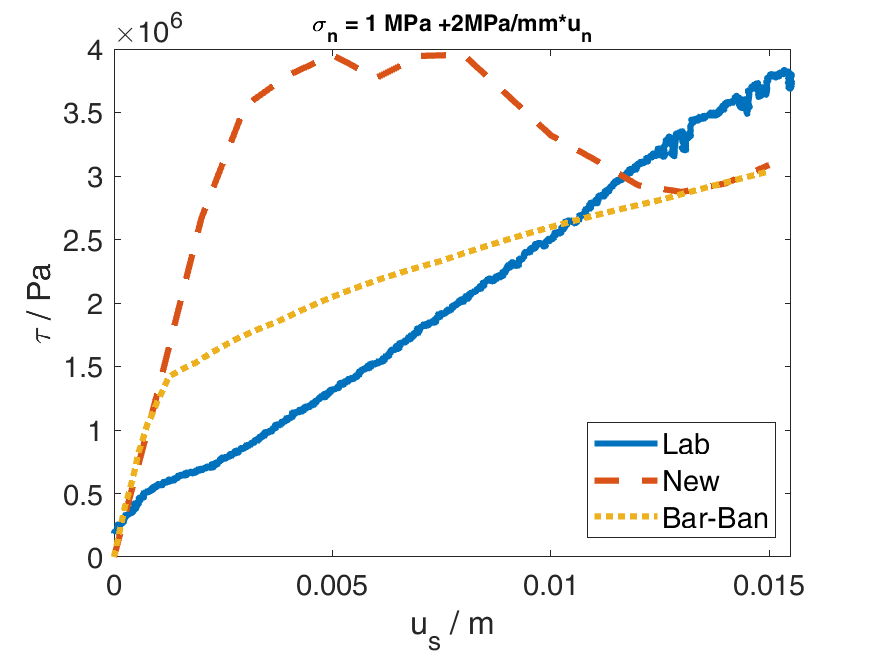
\includegraphics[width=0.99\textwidth]{./figures/MEX3-2_2ShearCurveOrig.png}
\subcaption{Original geometry}
%\label{fig:}
\end{subfigure}
\begin{subfigure}[c]{0.48\textwidth}
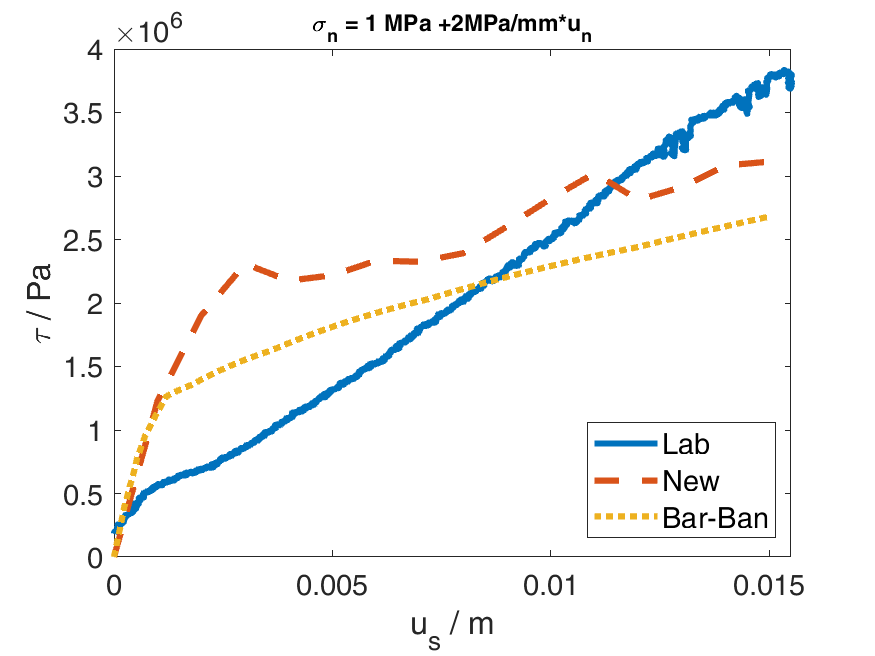
\includegraphics[width=0.99\textwidth]{./figures/MEX3-2_2ShearCurveWithout.png}
\subcaption{Adapted geometry}
%\label{fig:}
\end{subfigure}
\caption{Shear curves for $K_n=2.0\,\unit{MPa}$}
\label{fig:MEX3_2_2ShearCurve}
\end{figure}

\begin{figure}
\begin{subfigure}[c]{0.48\textwidth}
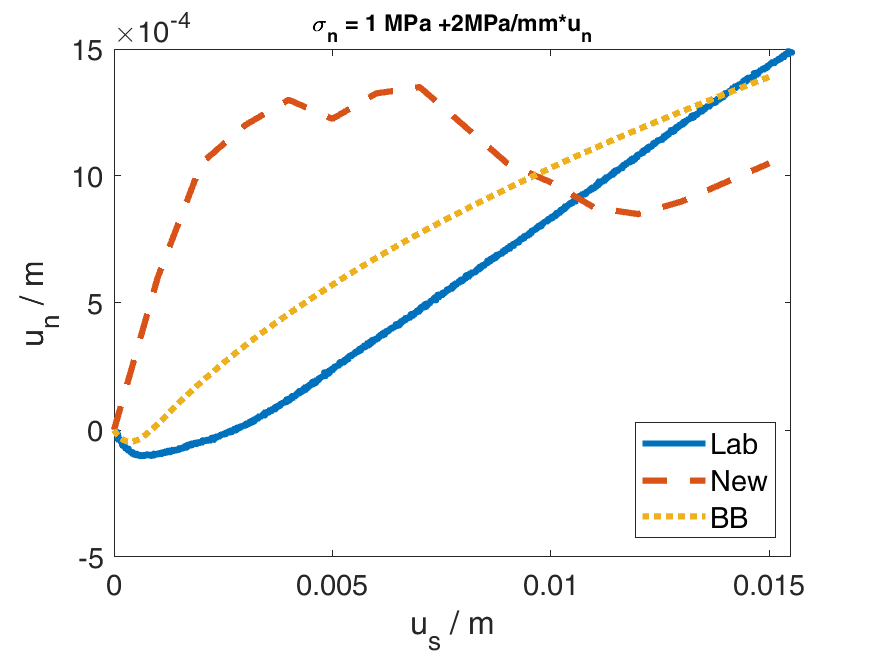
\includegraphics[width=0.99\textwidth]{./figures/MEX3-2_2DilationOrig.png}
\subcaption{Original geometry}
%\label{fig:}
\end{subfigure}
\begin{subfigure}[c]{0.48\textwidth}
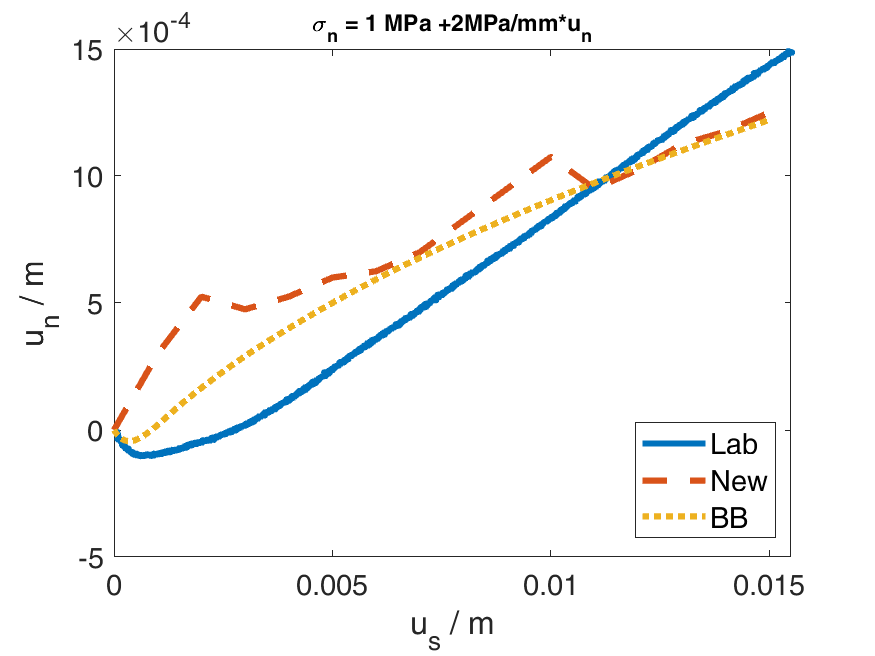
\includegraphics[width=0.99\textwidth]{./figures/MEX3-2_2DilationWithout.png}
\subcaption{Adapted geometry}
%\label{fig:}
\end{subfigure}
\caption{Dilatation curves for $K_n=2.0\,\unit{MPa}$}
\label{fig:MEX3-2_2Dilation}
\end{figure}

In Fig. \ref{fig:MEX3_2_2ShearCurve} and Fig. \ref{fig:MEX3-2_2Dilation} the shear and dilatation curves for a higher stiffness can be seen. Now the stiffness dominates the normal stress and consequently the shear stress. That's why the curves for shear stress and dilatation have a similar shape. In this case the adapted geometry improves the quality of the results fairly though it is not perfect. The main difference is that in the laboratory tests in the beginning of a shear test a compaction or settlement of the rock joint is observed. This is caused by imperfect matching of the two parts of the rock sample. The new code uses just one surface with a perfectly fitting counterpart. The result is the over prediction of the shear stress in the beginning stage of the shear test. For the original geometry this effect is more pronounced than for the adapted geometry.\\
As a conclusion it can be said that the dilatation modelling is the key point to model CNS tests. With increasing stiffness values this dependency becomes more and more important. The pure geometric approach delivers results in the correct magnitude but it is still difficult to forecast how big the difference will be. By carefully inspecting all available information and using them the overall result quality could be increased significantly.\\